%!Tex Root = ../Tutorat1.tex
% ./Packete.tex
% ./Design.tex
% ./Deklarationen.tex
% ./Aufgabe2.tex
% ./Aufgabe3.tex
% ./Bonus.tex

\section{Task 1 - Memory map}

\begin{frame}{Task 1 - Memory Map}{Task 1.1}
  \begin{solution}
    \begin{columns}
      \begin{column}{0.2\textwidth}
        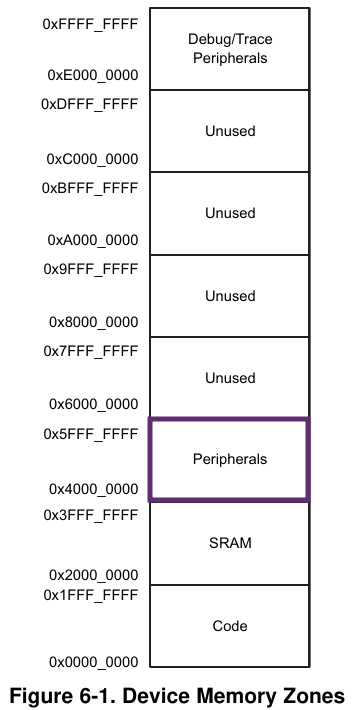
\includegraphics[height=0.5\paperheight]{./figures/peripherals.png}
      \end{column}
      \begin{column}{0.8\textwidth}
        \begin{itemize}
          \item $0x5FFF\_FFFF - 0x4000\_0000 + 1 = 0x2000\_0000$
          \item $0x2000\_0000 = 2 \cdot 16^7 = 2 \cdot {(2^4)}^7 = 2 \cdot 2^{4\cdot 7} = 2^{1+28} = 2^{29}$
        \end{itemize}
      \end{column}
    \end{columns}
  \end{solution}
\end{frame}

\begin{frame}{Task 1 - Memory Map}{Task 1.1}
  \begin{solution}
    \begin{columns}
      \begin{column}{0.4\textwidth}
        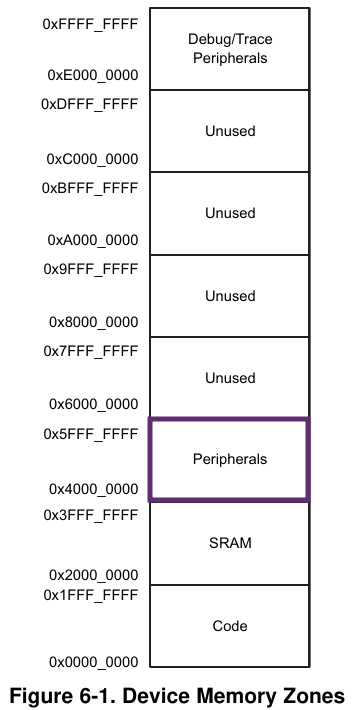
\includegraphics[height=0.5\paperheight]{./figures/peripherals.png}
        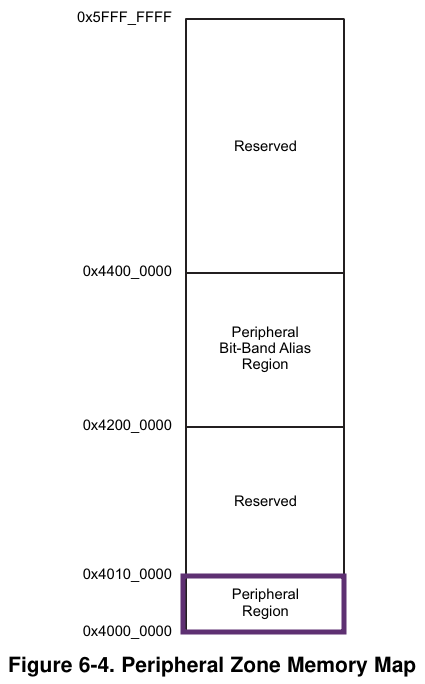
\includegraphics[height=0.5\paperheight]{./figures/peripherals_region.png}
      \end{column}
      \begin{column}{0.6\textwidth}
        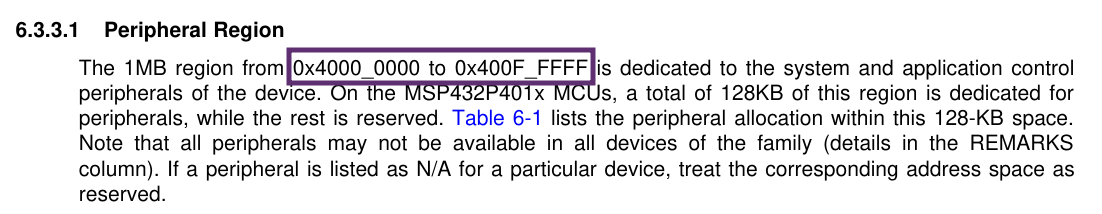
\includegraphics[width=0.5\paperwidth]{./figures/system_and_application_control_peripherals.png}
        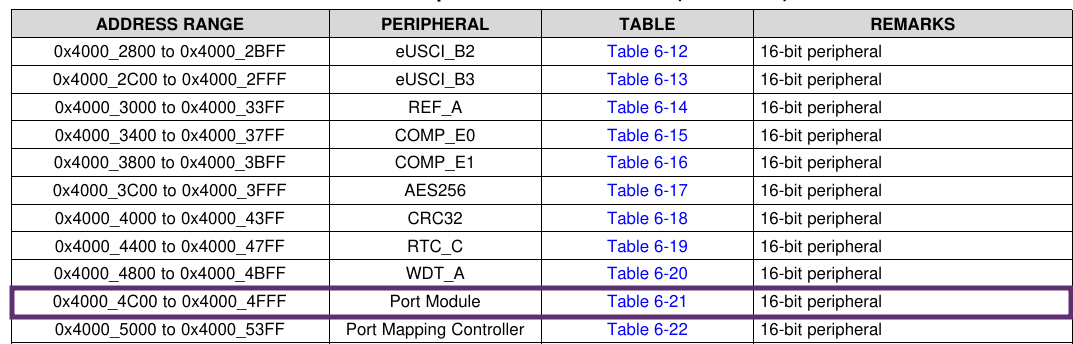
\includegraphics[width=0.5\paperwidth]{./figures/port_module.png}
      \end{column}
    \end{columns}
    \begin{itemize}
      \item $0x4000\_4FFF - 0x4000\_4C00 + 1 = 0x0400$
      \item $0x0400 = 4 \cdot 16^2 = 2^2 \cdot {(2^4)}^2 = 2^2 \cdot 2^{(4\cdot 2)} = 2^{2+8} = 2^{10}$
    \end{itemize}
  \end{solution}
\end{frame}

\if\preview0{
\begin{frame}[allowframebreaks]{Task 1 - Memory Map}{Task 1.1}
  \begin{solution}
    \begin{columns}
      \begin{column}{0.4\paperwidth}
        \centering
        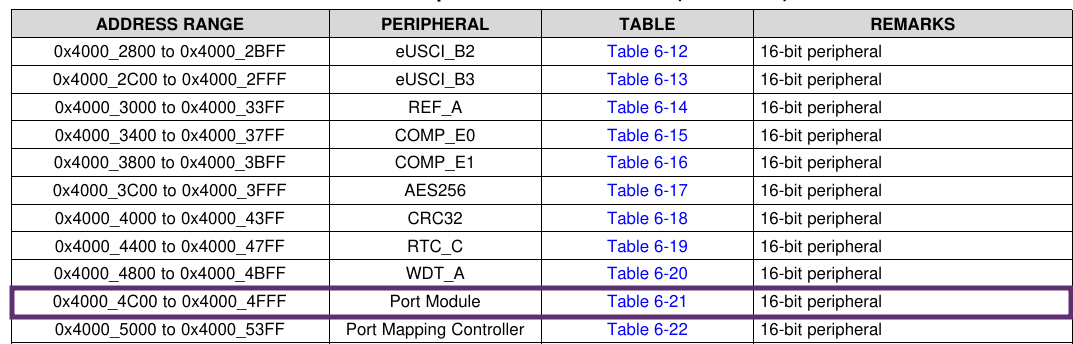
\includegraphics[width=0.3\paperwidth]{./figures/port_module.png}
        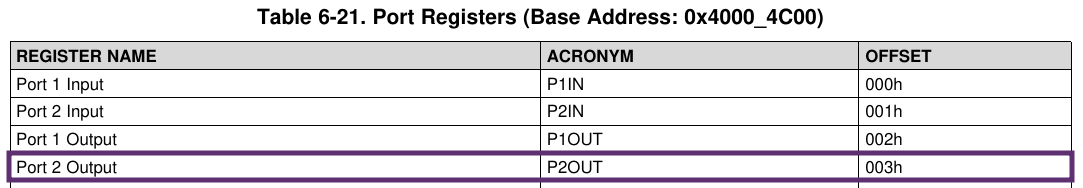
\includegraphics[width=0.3\paperwidth]{./figures/port2.png}
        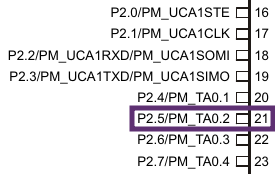
\includegraphics[height=0.2\paperheight]{./figures/2_5.png}
      \end{column}
      \begin{column}{0.6\paperwidth}
        \begin{itemize}
          \item $0x4000\_4C00 + 0x0003 = 0x4000\_4C03$
          \item 6th last significant bit $\Rightarrow$ $0b0010\_0000$
        \end{itemize}
      \end{column}
    \end{columns}
  \end{solution}
  \begin{Sidenote}
    \begin{itemize}
      \item 003h is an alternative way to wite 0x0003
    \end{itemize}
  \end{Sidenote}
\end{frame}

\begin{frame}[allowframebreaks]{Task 1 - Memory Map}{Task 1.1\vspace{0.25cm}}
  \begin{solution}
    \begin{columns}
      \begin{column}{0.3\paperwidth}
        \centering
        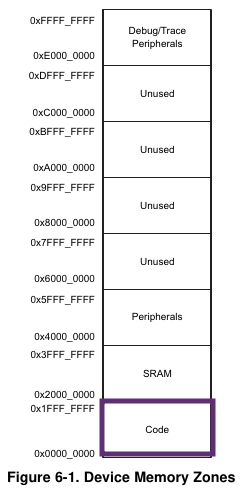
\includegraphics[height=0.4\paperheight]{./figures/code.png}
        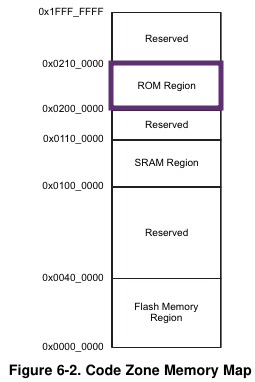
\includegraphics[height=0.4\paperheight]{./figures/rom.png}

      \end{column}
      \begin{column}{0.7\paperwidth}
        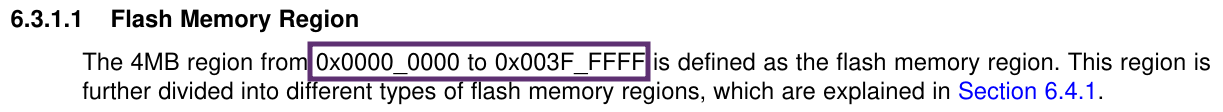
\includegraphics[height=0.095\paperheight]{./figures/rom2.png}
        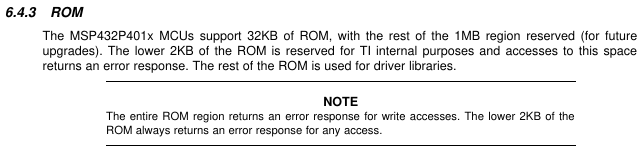
\includegraphics[height=0.25\paperheight]{./figures/rom3.png}
      \end{column}
    \end{columns}
    \begin{itemize}
      \item $0x020F\_FFFF - 0x0200\_0000 + 1 = 0x0010\_0000$.
      \item $16^5 = {(2^4)}^5 = 2^{4\cdot 5} = 2^{20} \text{addresses}$
    \end{itemize}
  \end{solution}
  \begin{solution}
    \begin{itemize}
      \item each address location corresponds to \alert{one byte} $\Rightarrow$ \alert{addressable memory space} is $2^{20} Byte$ or $1 MiB$.
      \item number of 4-byte words is a \alert{quarter} of that, which is $\frac{2^{20} Byte}{2^2} = 2^{18} words = 2^8 Kiwords= 256 Kiwords$
    \end{itemize}
  \end{solution}
  \begin{Sidenote}
    \begin{itemize}
      \item developer can not write to these addresses, only the manufacturer can (ROM = \alert{R}ead-\alert{o}nly \alert{m}emory)
      \item the MSP432P401x MCUs supports 32KB of ROM, and the rest of the 1MByte ROM region is reserved for \alert{future upgrades}
    \end{itemize}
  \end{Sidenote}
\end{frame}
}\fi

\begin{frame}{Task 1 - Memory Map}{Task 1.2\vspace{0.25cm}}
  \begin{figure}
    \centering
    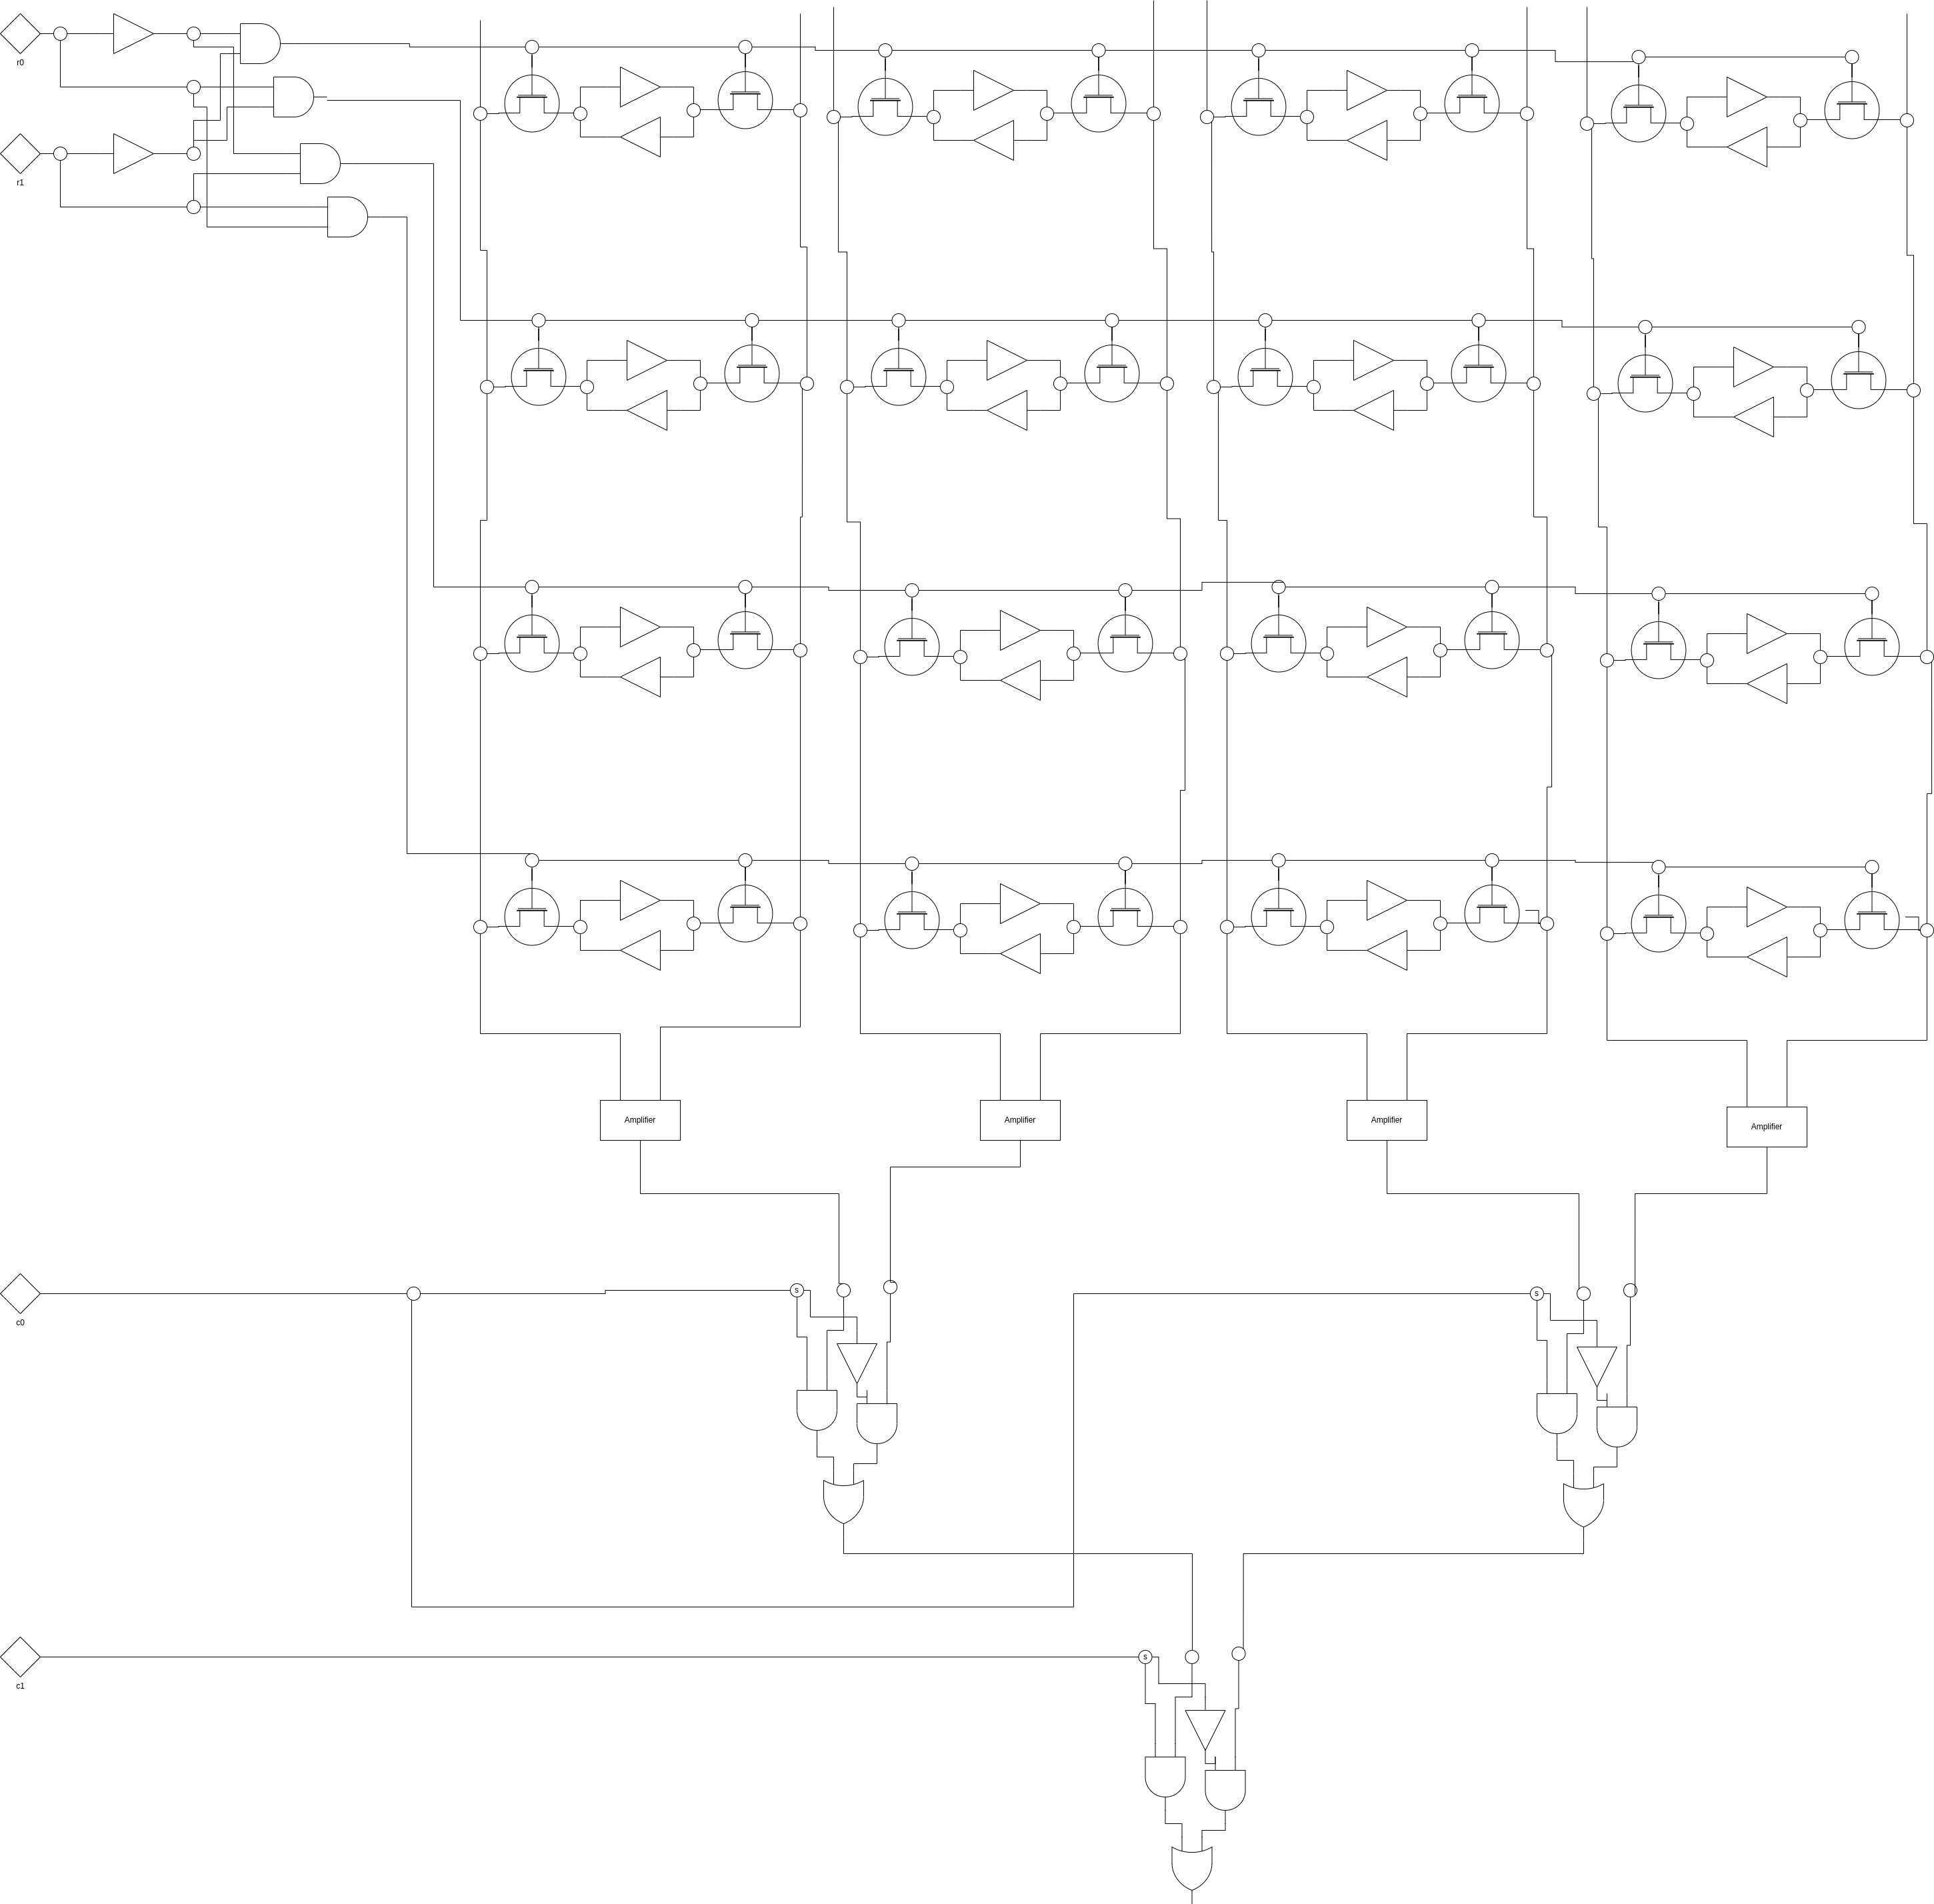
\includegraphics[height=0.6\paperheight]{./figures/sram.png}
    \caption{SRAM-cell array}
  \end{figure}
\end{frame}

\begin{frame}{Task 1 - Memory Map}{Task 1.2\vspace{0.25cm}}
  \begin{itemize}
    \item $u$ \alert{row} select bits and $w$ \alert{column} select bits
    \item \alert{we need:}
    \begin{itemize}
      \item $2^{(u+w)}$ memory cells
      \item one $u$-bit decoder
      \item one $2^w$-to-$1$ multiplexer
      \item $2^w$ sense amplifiers
    \end{itemize}
  \end{itemize}
\end{frame}


\begin{frame}[allowframebreaks]{Task 1 - Memory Map}{Task 1.2\vspace{0.25cm}}
  \begin{figure}
    \centering
    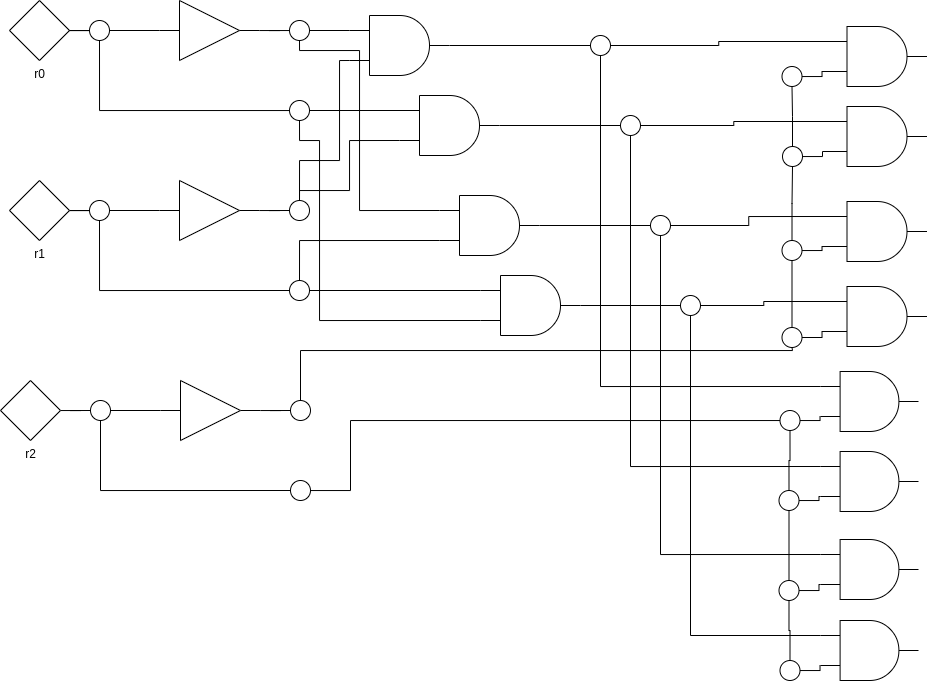
\includegraphics[height=0.6\paperheight]{./figures/3BitDecoder.png}
    \caption{3-Bit Decoder}
  \end{figure}
  \begin{figure}
    \centering
    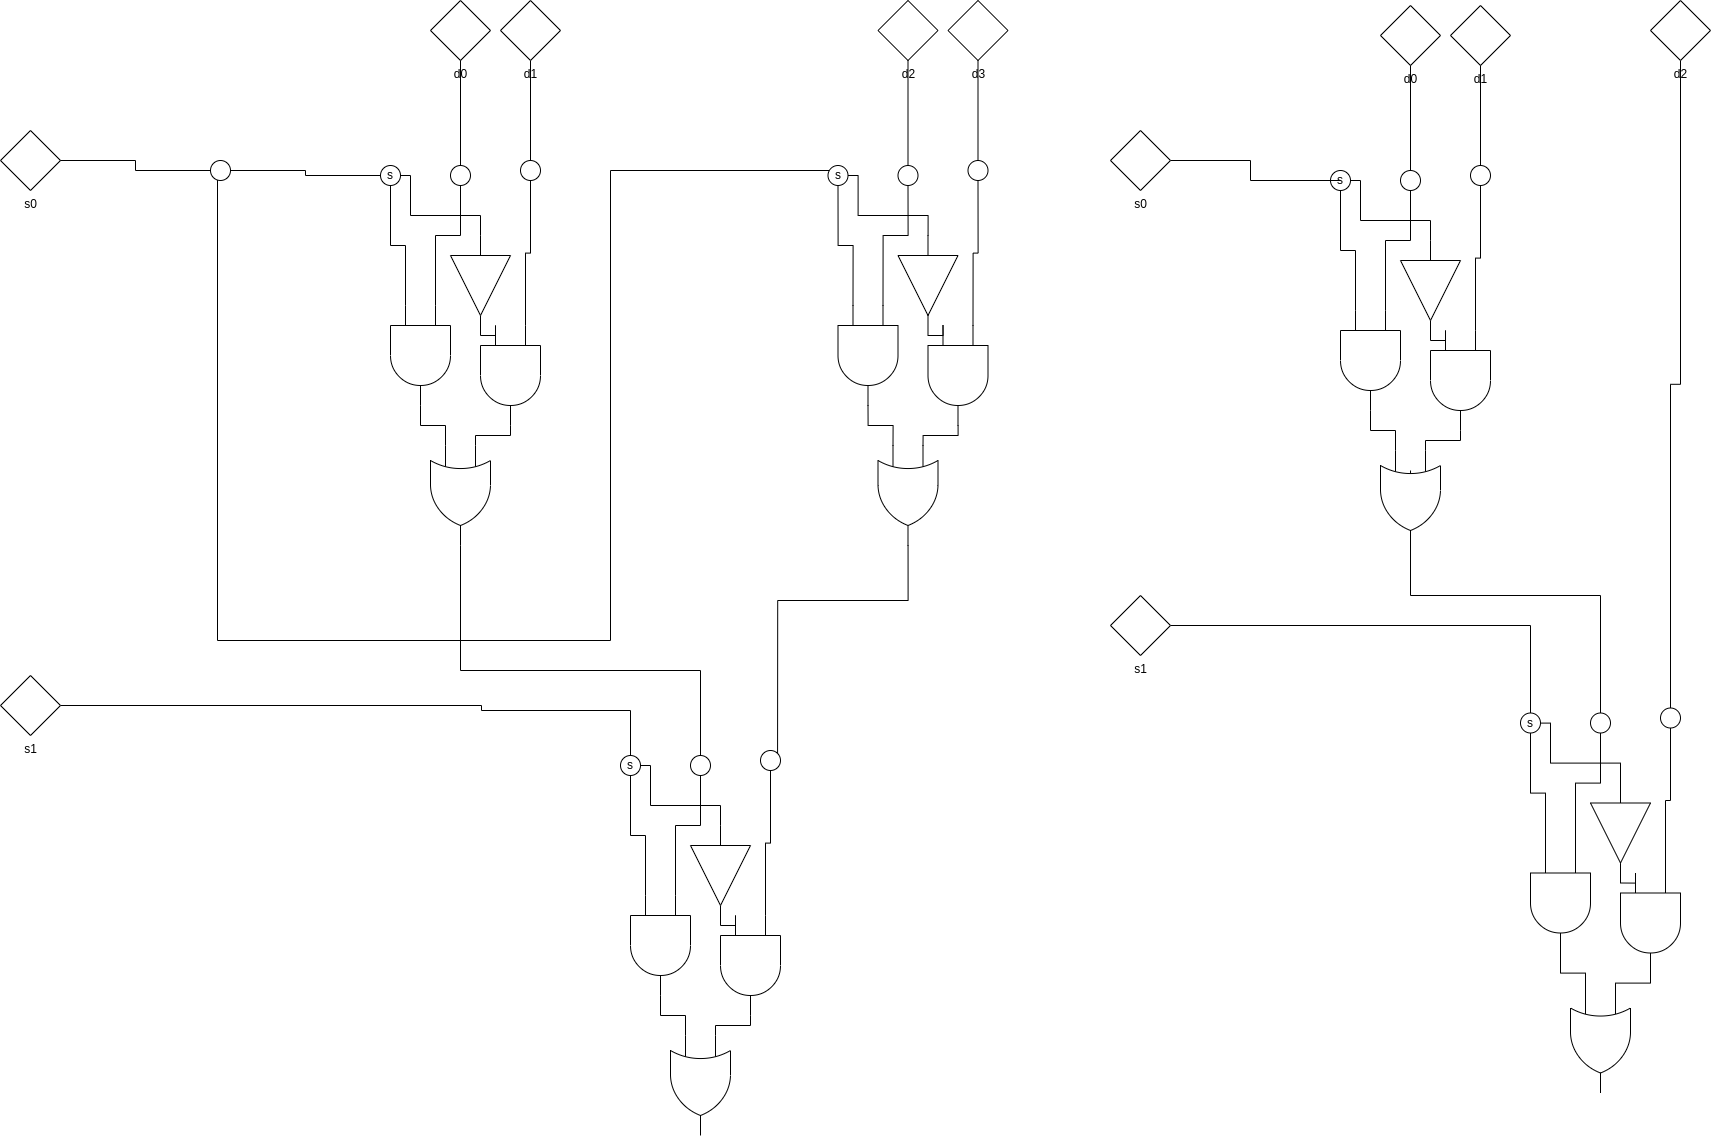
\includegraphics[height=0.6\paperheight]{./figures/3_to_1_multiplexer.png}
    \caption{4-to-1 and 3-to-1 Multiplexer}
  \end{figure}
\end{frame}

\if\preview0{
\begin{frame}[allowframebreaks]{Task 1 - Memory Map}{Task 1.2\vspace{0.25cm}}
  \begin{itemize}
    \item \alert{memory cell area:}
    \begin{itemize}
      \item for a $8$-\alert{bit address}, we need $28$ \alert{memory cells}.
      \item $C=2^8 \cdot A_{\mathrm{mem}}=2^8 \cdot 6=1536$.
    \end{itemize}
    \item \alert{$u$-bit decoder area:}
    \begin{itemize}
      \item for activating one of the $2^u$ \alert{word lines}.
      \item we construct a $k$-bit decoder using $2$ \alert{smaller decoders} and $2^k$ $2$-input \alert{AND gates}.
      \item the \alert{smaller decoders} should be of size $\frac{k}{2}$ if $k$ is \alert{even}, or of sizes $\frac{k + 1}{2}$ and $\frac{k - 1}{2}$ if $k$ is \alert{odd}.
      \item $D(k)= \begin{cases}A_{\mathrm{NOT}} & \text { if } k=1 \\ 2 \cdot D\left(\frac{k}{2}\right)+A_{\mathrm{AND}} \cdot 2^k & \text { if } k>1 \text { and } k \text { is even } \\ D\left(\frac{k-1}{2}\right)+D\left(\frac{k+1}{2}\right)+A_{\mathrm{AND}} \cdot 2^k & \text { if } k>1 \text { and } k \text { is odd }\end{cases}$
    \end{itemize}
    \item \alert{$2w$-to-$1$ multiplexer area:}
    \begin{itemize}
      \item  for selecting one of the $2^w$ \alert{bit lines}.
      \item  we can construct a $2^k$-to-$1$ \alert{multiplexer} for any $k$ using two $2^{k-1}$-to-$1$ \alert{multiplexers} and one $2$-to-$1$ \alert{multiplexer}.
      \item $M(k)= \begin{cases}A_{\operatorname{mux}} = 4 & \text { if } k=1 \\ 2 \cdot M(k-1)+A_{\operatorname{mux}} & \text { otherwise }\end{cases}$.
    \end{itemize}
    \item \alert{single sense amplifier area:}
    \begin{itemize}
      \item for each of the $w$ \alert{column bit lines}
      \item $S(w)=2^w \cdot A_{\text {sense}}$
    \end{itemize}
    \item there are $8$ possible \alert{implementations} for $u$ and $w$
    \item the area \alert{excluding} the memory cells: D(u) + M (w) + S(w)
  \end{itemize}
\end{frame}

\begin{frame}{Task 1 - Memory Map}{Task 1.2\vspace{0.25cm}}
  \centering
 \begin{table}
   \begin{tabular}{|c|c||c|c|c|c|}
      \hline$u$ & $w$ & Decoder $D(u)$ & Multiplexer $M(w)$ & Sense Amp $S(w)$ & Total \\
      \hline \hline 0 & 8 & 0 & 1020 & 1280 & 2300 \\
      \hline 1 & 7 & 1 & 508 & 640 & 1149 \\
      \hline 2 & 6 & 6 & 252 & 320 & 578 \\
      \hline 3 & 5 & 15 & 124 & 160 & 299 \\
      \hline 4 & 4 & 28 & 60 & 80 & 168 \\
      \hline 5 & 3 & 53 & 28 & 40 & 121 \\
      \hline 6 & 2 & 94 & 12 & 20 & 126 \\
      \hline 7 & 1 & 171 & 4 & 10 & 185 \\
      \hline 8 & 0 & 312 & 0 & 5 & 317 \\
      \hline
    \end{tabular}
    \caption{Different SRAM implementations}
 \end{table}
\end{frame}
}\fi
